% =====================================================================
%  TikZ-Stile fuer die Topologie-Abbildungen (Kapitel 2).
%  Wird einmal in der Praeambel von thesis.tex geladen.
%  Die Abbildungen selbst erzeugt abbildungen/gen_topologie_figuren.py.
% =====================================================================
\usetikzlibrary{arrows.meta, positioning, fit, backgrounds}

\definecolor{topoNode}{HTML}{E8EDF2}   % neutrale Knoten
\definecolor{topoLine}{HTML}{5A6672}   % Rahmen und Erreichbarkeitskanten
\definecolor{topoEntry}{HTML}{FFE0B2}  % Einstiegsknoten
\definecolor{topoCJ}{HTML}{F8C9C4}     % Crown Jewel
\definecolor{topoDC}{HTML}{D6E4F0}     % Domain Controller
\definecolor{topoCred}{HTML}{B03A2E}   % Credential-Kanten

\tikzset{
  topofig/.style={
    every node/.append style={font=\scriptsize},
    >={Stealth[length=4pt]},
  },
  netnode/.style={
    draw=topoLine, line width=0.4pt, fill=topoNode, rounded corners=2pt,
    align=center, inner sep=2.5pt, minimum width=17mm, minimum height=7mm,
  },
  entrynode/.style={netnode, fill=topoEntry, line width=0.8pt},
  cjnode/.style={netnode, fill=topoCJ, line width=0.8pt},
  dcnode/.style={netnode, fill=topoDC},
  % Strukturell nie erreichbare Knoten: blass und gestrichelt umrandet.
  isolated/.style={draw=topoLine!55, dashed, fill=topoNode!45, text=black!55},
  reach/.style={draw=topoLine, line width=0.5pt, ->},
  cred/.style={draw=topoCred, line width=0.5pt, densely dashed, ->},
  dcbadge/.style={font=\tiny\itshape, text=topoLine, inner sep=1pt},
}

% Legende, damit sie nicht in jeder Abbildung wiederholt werden muss.
\newcommand{\topolegende}{%
  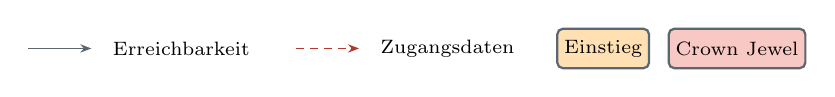
\begin{tikzpicture}[topofig, baseline]
    \draw[reach] (0,0) -- (0.8,0);
    \node[anchor=west, font=\scriptsize] at (0.95,0) {Erreichbarkeit};
    \draw[cred] (3.4,0) -- (4.2,0);
    \node[anchor=west, font=\scriptsize] at (4.35,0) {Zugangsdaten};
    \node[entrynode, minimum width=11mm, minimum height=5mm] at (7.3,0) {Einstieg};
    \node[cjnode, minimum width=11mm, minimum height=5mm] at (9.0,0) {Crown Jewel};
  \end{tikzpicture}%
}
